
\medskip

%L'image ci-dessous représente la position obtenue au déclenchement du bloc départ
%d'un programme de jeu.
%
%\medskip
%
%\parbox{0.55\linewidth}{\psset{unit=0.5cm}
%\begin{pspicture*}(-6,-4)(6,4)
%\multido{\n=-6+1}{13}
%{
%\multido{\na=-4+1}{9}{\psdots[dotscale=0.5](\n,\na)}
%}
%\psaxes[Dx=10,Dy=10]{->}(0,0)(-6,-4)(6,4)
%\uput[dl](0,0){O}
%\psdots[dotscale=2.5](4,3)
%\rput(-3,-2){Chat}
%\end{pspicture*}}
%\hfill
%\parbox{0.43\linewidth}{L'arrière-plan est constitué de points
%espacés de 40 unités.
%
%Dans cette position, le chat a pour
%coordonnées $(- 120~;~ -80)$.
%
%\textbf{Le but du jeu est de positionner le
%chat sur la balle.}}
%
%\medskip

\begin{enumerate}
\item %Quelles sont les coordonnées du centre de la balle représentée dans cette position ?
Le centre de la balle a pour coordonnées (160~;~120).
\item %Dans cette question, le chat est dans la position obtenue au déclenchement du bloc
%départ.

%Voici le script du lutin \og chat \fg{} qui se déplace.

\parbox{0.4\linewidth}{\textbf{a.} %Expliquez pourquoi le chat ne revient pas à sa position
%de départ si le joueur appuie sur la touche $\to$ puis sur la touche $\gets$.
Vers la droite il y a déplacement de 80 unités alors que vers la gauche on de déplace de 40 unités.
\textbf{b.} %Le joueur appuie sur la succession de touches
%suivante : $\to$ $\to$  $\uparrow$ $\gets$ $\downarrow$.

%Quelles sont les coordonnées $x$ et $y$ du chat après ce déplacement ?
Horizontalement le déplacement est de : $2 \times 80 - 1 \times 40 = 160 - 40 = 120$ et verticalement : $1 \times 80 - 1 \times 40 = 80 - 40 = 40$.

Le chat est donc au point de coordonnées $(0~;~- 40)$.
\textbf{c.} Parmi les propositions de succession de touches ci-dessous, laquelle permet au
chat d'atteindre la balle ?} \hfill 
\parbox{0.58\linewidth}{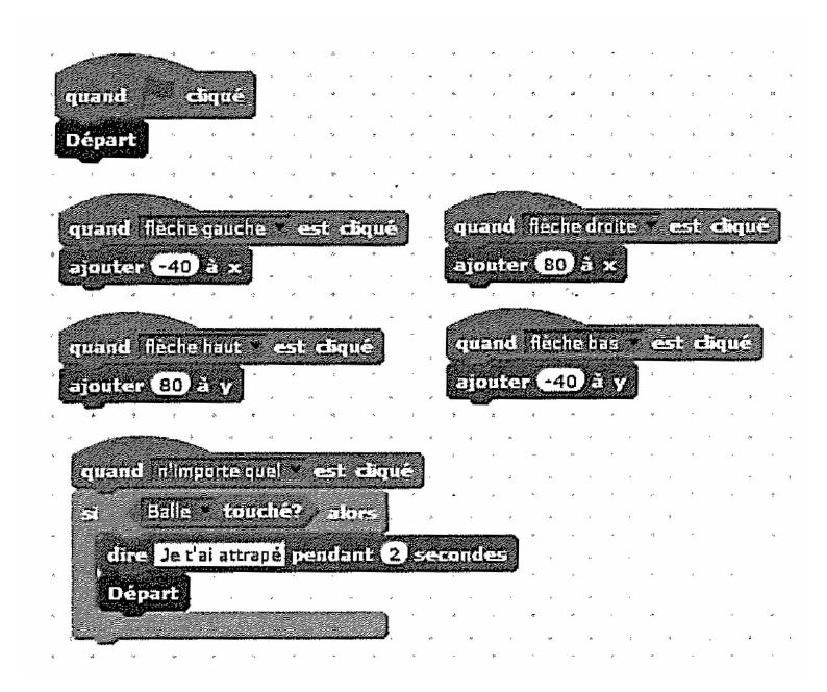
\includegraphics[width=6cm]{ScratchAmduNord2017.eps}}

\begin{tabularx}{\linewidth}{|*{3}{>{\centering \arraybackslash}X|}}\hline
Déplacement 1 &Déplacement 2 &Déplacement 3\\ \hline
$\to \to \to \to \to \to \to \uparrow\uparrow\uparrow\uparrow\uparrow$&$\to\to\to \uparrow\uparrow\uparrow \to \downarrow \gets$&$\uparrow \to \uparrow \to \uparrow \to \to \downarrow \downarrow$\\ \hline
$7 \times 80 = 560$ &$4\times 80 - 1\times 40 = 280$&$4 \times 80 = 320$\\
horizontalement&horizontalement&horizontalement\\
$5 \times 80 = 400$ &$3\times 80 - 1\times 40 = 200$&$3 \times 80 - 2\times 40 = 160$\\
verticalement&verticalement&verticalement\\
arrivée en (440~;~320)&arrivée en (160~;~120)&arrivée en (200~;~80)\\ \hline
\end{tabularx}

C'est donc le déplacement 2.
\item %Que se passe-t-il quand le chat atteint la balle ?
Quand le chat atteint la balle il s'affiche pendant 2 secondes : \og Je t'ai attrapé \fg.
\end{enumerate}

\vspace{0,5cm}

